\documentclass[11pt,a4paper]{article}

% === Encoding & Fonts ===
\usepackage[utf8]{inputenc}
\usepackage[T1]{fontenc}
\usepackage{lmodern}

% === Page Layout ===
\usepackage[margin=1in]{geometry}

% === Math ===
\usepackage{amsmath,amssymb}

% === Graphics & Tables ===
\usepackage{graphicx}
\usepackage{booktabs}
\usepackage{multirow}
\usepackage{tabularx}
\usepackage{colortbl}
\usepackage{xcolor}

% === Figures ===
\usepackage{float}
\usepackage{subcaption}

% === Code Listings ===
\usepackage{listings}
\lstset{
  basicstyle=\ttfamily\small,
  breaklines=true,
  frame=single,
  numbers=left,
  numberstyle=\tiny\color{gray},
}

% === Hyperlinks ===
\usepackage[colorlinks=true,linkcolor=blue,citecolor=blue,urlcolor=blue]{hyperref}

% PDF document properties. Without these hyperref emits an empty /Title, so
% search engines indexing the hosted PDF fall back to the filename
% ("realvuln-paper.pdf") as the result headline. Kept as plain text: the PDF
% string is not TeX, so \realvuln{} and the \\ line break do not belong here.
\hypersetup{
  pdftitle={RealVuln: An Open Benchmark for Evaluating Security Scanners on Real-World Code},
  pdfauthor={Faizan Raza; John Pellew},
  pdfsubject={Security scanner benchmarking; static analysis; vulnerability detection},
  pdfkeywords={RealVuln, benchmark, SAST, vulnerability detection, LLM security scanners, F3 score},
}

% === Citations ===
\usepackage[numbers,sort&compress]{natbib}

% === TODOs (remove before submission) ===
\usepackage[textsize=small,color=yellow!40]{todonotes}

% === Compact Lists ===
\usepackage{enumitem}
\setlist{nosep}

% === Header/Footer ===
\usepackage{fancyhdr}
\pagestyle{fancy}
\fancyhf{}
\rhead{\thepage}
\lhead{RealVuln Benchmark}

% === Custom Commands ===
\newcommand{\realvuln}{\textsc{RealVuln}}
\newcommand{\fscore}[1]{F\textsubscript{#1}}
\newcommand{\ftwoscore}{\fscore{2}}
\newcommand{\fonescore}{\fscore{1}}
\newcommand{\fhalfscore}{\fscore{0.5}}

% === Metadata ===
\title{\realvuln{}: An Open Benchmark for Evaluating\\Security Scanners on Real-World Code}
\author{
  Faizan Raza\thanks{Kolega AI} \\
  \texttt{faizan@kolega.ai}
  % Add co-authors here
}
\date{\today}

\begin{document}

\maketitle

\begin{abstract}
How do security scanners compare when evaluated on real-world code? We
present \textsc{RealVuln}, the first open-source benchmark that
systematically compares three categories of vulnerability scanners---rule-based
SAST, general-purpose LLMs, and security-specialized systems---across 26
real-world Python repositories containing 796 hand-labeled entries (676 vulnerabilities and
120 false-positive traps). We evaluate 15 scanners (3 rule-based SAST
tools, 10 general-purpose LLM configurations, and 2 security-specialized
systems) using the recall-weighted F3 score ($\beta{=}3$, recall weighted 9$\times$ over precision) as the primary metric. Our
results reveal a clear three-tier hierarchy: the security-specialized
scanner (Kolega, F3\,=\,73.0) substantially outperforms the best
general-purpose LLM (Claude Sonnet~4.6, F3\,=\,51.7), which in turn
outperforms the best rule-based SAST tool (Semgrep, F3\,=\,17.7) by
nearly 3$\times$. All code,
ground-truth data, scanner outputs, and scoring scripts are released
under an open-source license. An interactive dashboard is available at \url{https://realvuln.kolega.dev/}. \textsc{RealVuln} is designed as a living
benchmark---versioned, community-driven, and with a roadmap toward
multi-language coverage.

\end{abstract}

\section{Introduction}

Static Application Security Testing (SAST) tools are a cornerstone of secure
software development, yet their practical value is undermined by noise.
The Ghost Security CAST report found a 99.5\% false positive rate for
command-injection findings in Python/Flask applications, with 91\% of all
2{,}166 findings across categories classified as noise~\cite{ghost2025cast}.
The picture is similar at scale: NIST's SATE~V and SATE~VI evaluations
measured false positive rates of 70--92\% depending on language and
tool~\cite{delaitre2018satev,delaitre2023satevi}. On the detection side,
the Fluid Attacks benchmark showed that the best fully automated tool found
only 22.7\% of known vulnerabilities, with an average F-score of 1.9\%
across 36 commercial and open-source scanners~\cite{fluidattacks2025}.
Practitioners, faced with hundreds of alerts they must manually triage,
increasingly ignore scanner output altogether.

A new generation of LLM-powered security scanners promises to change this.
By leveraging large language models for semantic code understanding rather than
pattern matching, these tools claim deeper reasoning about data flow, context,
and exploitability. Yet no open benchmark exists to verify whether LLM-based
scanners actually deliver on these promises---or whether they simply trade one
set of failure modes for another. Existing benchmarks fall short on one or more
critical dimensions:

\begin{itemize}
  \item \textbf{Synthetic code.} The OWASP Benchmark~\cite{owaspbenchmark}
    consists of synthetic Java test cases that do not reflect the structure,
    complexity, or idioms of real-world applications.
  \item \textbf{Closed data.} SastBench~\cite{feiglin2026sastbench} is the
    closest prior work to ours, but its dataset has not been publicly released
    and its evaluation focuses on triage agents rather than scanner accuracy.
  \item \textbf{Vendor self-assessment.} Benchmarks published by
    ZeroPath~\cite{zeropath2024}, Cycode~\cite{cycode2024benchmark}, and
    DryRun~\cite{dryrun2025sast} evaluate their own tools on proprietary
    datasets, making independent reproduction impossible.
  \item \textbf{No false positive measurement.} Most benchmarks report
    detection rates alone, ignoring the false positive burden that dominates
    practitioner experience.
\end{itemize}

\noindent
We expand on these limitations in Section~\ref{sec:related-work}. The gap is
clear: the community lacks a reproducible, open benchmark that tests both
traditional and LLM-based scanners on real code, measuring not just what they
find but also what they falsely flag.

This paper makes three contributions:

\begin{enumerate}
  \item \textbf{RealVuln}, the first fully open-source SAST benchmark built
    from real-world code. It comprises 26 intentionally vulnerable Python
    repositories with 796 hand-labeled findings---including 120 false positive
    traps---scored using an F3-weighted metric ($\beta{=}3$, recall weighted 9$\times$ over precision) as the primary metric for production-grade security assessment, with F2 ($\beta{=}2$) reported as a secondary metric for lower-risk contexts.
  \item \textbf{The first large-scale head-to-head comparison} of 15 security
    scanners on identical ground truth: 3 traditional SAST tools (Semgrep,
    Snyk, SonarQube), 11 LLM-based scanner configurations spanning 7 model families, and
    1 proprietary hybrid system.
  \item \textbf{A living benchmark} with versioned scoring, a public
    dashboard, and a clear contribution path so that the community can add new
    scanners, repositories, and ground-truth labels over time.
\end{enumerate}

We release all code, ground-truth data, scanner results, scoring tooling, and
the interactive dashboard at
\url{https://github.com/kolega-ai/RealVulnBenchmark}.

\section{Background \& Related Work}
\label{sec:related-work}

Table~\ref{tab:benchmark-comparison} summarizes how RealVuln relates to prior
benchmarks across seven desirable properties. We discuss each category of prior
work below, highlighting the specific gaps that motivated our design.

%% ── Comparison table ─────────────────────────────────────────────────────────
\begin{table*}[t]
\caption{Comparison of SAST benchmarks. \emph{Real Code}: uses unmodified
  application source, not synthetic snippets. \emph{Open Data}: ground truth
  and scanner results publicly available. \emph{Open Scoring}: scoring code
  released for reproduction. \emph{FP Testing}: explicitly measures false
  positives. \emph{Multi-Scanner}: evaluates $\geq$3 scanners head-to-head.
  \emph{LLM Scanners}: includes LLM-based tools. \emph{Multi-Lang}: covers
  more than one programming language.}
\label{tab:benchmark-comparison}
\centering
\footnotesize
\begin{tabular}{@{}lccccccc@{}}
\toprule
\textbf{Benchmark} & \textbf{Real} & \textbf{Open} & \textbf{Open} & \textbf{FP} & \textbf{Multi-} & \textbf{LLM} & \textbf{Multi-} \\
 & \textbf{Code} & \textbf{Data} & \textbf{Scoring} & \textbf{Test} & \textbf{Scanner} & \textbf{Scan.} & \textbf{Lang} \\
\midrule
OWASP Benchmark~\cite{owaspbenchmark}
  & $\times$ & \checkmark & \checkmark & \checkmark & \checkmark & $\times$ & $\times$ \\
Juliet Test Suite~\cite{boland2012juliet}
  & $\times$ & \checkmark & $\times$ & $\times$ & $\times$ & $\times$ & $\times$ \\
SastBench~\cite{feiglin2026sastbench}
  & \checkmark & $\times$ & $\times$ & \checkmark & $\times$ & $\times$ & \checkmark \\
ZeroPath/XBOW~\cite{zeropath2024}
  & $\times$ & $\sim$ & $\times$ & \checkmark & \checkmark & \checkmark & $\times$ \\
Fluid Attacks~\cite{fluidattacks2025}
  & \checkmark & $\times$ & $\times$ & \checkmark & \checkmark & $\times$ & $\times$ \\
CASTLE~\cite{dubniczky2025castle}
  & $\times$ & \checkmark & \checkmark & $\times$ & \checkmark & \checkmark & \checkmark \\
Cycode~\cite{cycode2024benchmark}
  & \checkmark & $\times$ & $\times$ & $\times$ & \checkmark & $\times$ & \checkmark \\
DryRun~\cite{dryrun2025sast}
  & \checkmark & $\sim$ & $\times$ & $\times$ & \checkmark & $\times$ & \checkmark \\
\midrule
\textbf{RealVuln (ours)}
  & \checkmark & \checkmark & \checkmark & \checkmark & \checkmark & \checkmark & $\times$ \\
\bottomrule
\end{tabular}
\end{table*}

%% ── §1  Synthetic benchmarks ────────────────────────────────────────────────
\paragraph{Synthetic benchmarks.}
The OWASP Benchmark~\cite{owaspbenchmark} (${\sim}$2{,}740 synthetic Java servlets) and the NIST Juliet Test Suite~\cite{boland2012juliet} (single-CWE C/C++/Java programs) are the most cited SAST evaluation suites. Both use short, self-contained test cases that let pattern-matching tools score well without understanding cross-file data flow or framework semantics, limiting their relevance to whole-application analysis.

%% ── §2  Unreleased datasets ─────────────────────────────────────────────────
\paragraph{Unreleased datasets.}
SastBench~\cite{feiglin2026sastbench} assembles 2{,}737 ground-truth samples across 38 languages from real CVEs, scored with the Matthews Correlation Coefficient. Its dataset is not publicly released, and it evaluates agentic \emph{triage} of SAST alerts rather than raw scanner detection accuracy. SastBench is complementary to RealVuln. It measures post-scan triage that we deliberately exclude, but cannot serve as an open benchmark for detection performance.

%% ── §3  Vendor benchmarks ───────────────────────────────────────────────────
\paragraph{Vendor benchmarks.}
ZeroPath~\cite{zeropath2024} published benchmark code and SARIF results as a public GitHub fork of the XBOW validation benchmarks, testing against major SAST vendors, a genuine step toward transparency, though without reusable scoring infrastructure or ground-truth labels. Fluid Attacks~\cite{fluidattacks2025} tested 36 scanners against a large JS/TS application (the best achieved 22.7\% recall), but neither the source nor the ground truth is public. Cycode~\cite{cycode2024benchmark} ran Bearer CLI against open-source projects and published raw classification data, but the methodology is not fully documented for reproduction. DryRun~\cite{dryrun2025sast} tested against public intentionally-vulnerable applications with per-vulnerability breakdowns, providing partial reproducibility. The shared limitation across all vendor benchmarks is a structural conflict of interest: each vendor selects the test conditions, interprets results, and lacks a unified framework for independent re-scoring.

%% ── §4  Dataset quality ─────────────────────────────────────────────────────
\paragraph{Dataset quality and label noise.}
Automated vulnerability datasets suffer from widespread label noise. Ding et al.~\cite{ding2024primevul} showed that a 7B model achieves 68\% F1 on BigVul but only 3\% on their cleaned PrimeVul dataset; CleanVul~\cite{li2025cleanvul} found over 40\% of entries in existing datasets mislabeled. CVEFixes~\cite{bhandari2021cvefixes} and ReposVul~\cite{wang2024reposvul} inherit the same tangled-commit problems. RealVuln takes the opposite position: 796 hand-labeled findings across 26 repositories, accepting lower scale in exchange for label quality that can be audited line by line.

%% ── §5  Agentic and LLM benchmarks ─────────────────────────────────────────
\paragraph{Agentic and LLM-oriented benchmarks.}
SWE-Bench~\cite{jimenez2024swebench} introduced the approach of evaluating AI agents on real GitHub issues with reproducible harnesses. SWE-Bench Verified~\cite{openai2025swebenchverified} further demonstrated the value of human-validated labels. CVE-Bench~\cite{zhu2025cvebench} measures whether agents can exploit real CVEs in containerized apps, highlighting knowledge-cutoff confounds. CASTLE~\cite{dubniczky2025castle} evaluates 25 tools (13 static analyzers, 10 LLMs, and 2 formal verification tools) on CWE detection but uses synthetic micro-benchmarks. Yildiz et al.~\cite{yildiz2025jitvul} found that agentic approaches outperformed function-level prompting for vulnerability detection but noted that agents still exhibit inconsistencies requiring further refinement.

%% ── §6  Honest self-critique ────────────────────────────────────────────────
\paragraph{Positioning and limitations of RealVuln.}
No prior benchmark systematically compares all three scanner
categories (Rule-Based SAST, General-Purpose LLMs, and Security-Specialized
systems) on identical ground truth. As Table~\ref{tab:benchmark-comparison}
shows, RealVuln is the only benchmark that simultaneously uses real code,
releases all data and scoring code, tests for false positives, and includes
scanners from all three categories.
We are forthright about its limitations in v1. First, RealVuln covers
Python only. This enables depth (Django, Flask, FastAPI, and raw Python
idioms are all represented), it cannot speak to scanner performance on memory-unsafe
languages or compiled ecosystems. Second, our ground truth covers only
OWASP-style application vulnerabilities (injection, XSS, authentication
flaws), but we do not yet include supply-chain, configuration, or
infrastructure-as-code findings. Third, we are ourselves a vendor (Kolega.Dev),
which creates the same conflict of interest we criticize above. We mitigate
this by open-sourcing \emph{everything}: ground truth labels, all scanner
result files, the scoring pipeline, and the interactive dashboard, so that any
researcher can audit, challenge, or extend our results. We view transparency
not as a defense against bias but as an invitation for the community to find it.

\section{Benchmark Design}
\label{sec:benchmark-design}

This section describes the design of \textsc{RealVuln}~v1.0: the taxonomy of target types it recognizes, how the dataset was constructed and labeled, the algorithm used to match scanner findings against ground truth, and the scoring metrics reported.

%% ----------------------------------------------------------------
\subsection{Target Type Taxonomy}
\label{sec:target-types}

We define five \emph{target types} to classify the code under test.
Version~1.0 of \textsc{RealVuln} covers only Type~1.

\medskip
\noindent\textbf{Type 1: Intentionally vulnerable applications.}
Open-source projects built \emph{on purpose} with security flaws for educational or CTF use (e.g., PyGoat, DVPWA, VAmPI).
These projects offer high vulnerability density and diverse CWE coverage, making them ideal for initial calibration.

\medskip
\noindent Types 2--5 (production CVEs, vulnerable libraries, benchmark roll-ups, and academic reproductions) are planned for future versions and defined precisely in the roadmap (Section~\ref{sec:living-benchmark}).

%% ----------------------------------------------------------------
\subsection{Dataset Construction}
\label{sec:dataset-construction}

\subsubsection{Repository Selection.}
We collected 26 intentionally vulnerable Python repositories from GitHub.
Selection criteria were: (1)~the project must be a multi-file application with a meaningful code structure (single-file toy scripts were excluded), (2)~the project must use a recognizable web framework, and (3)~the project should contribute CWE families not already saturated in the dataset.
Each repository is pinned to a specific commit SHA recorded in \texttt{benchmark-manifest.json}, ensuring that all scanners analyze identical source trees.

The 26~repositories span five web frameworks: Flask (15~repos), Django (3), FastAPI (3), aiohttp (1), and Tornado (1), with 3~repos using lightweight or custom HTTP stacks.
Table~\ref{tab:dataset-stats} summarizes the dataset.

\begin{table}[t]
  \centering
  \caption{Dataset statistics for \textsc{RealVuln}~v1.0.}
  \label{tab:dataset-stats}
  \footnotesize
  \begin{tabular}{@{}lr@{}}
    \toprule
    \textbf{Statistic} & \textbf{Value} \\
    \midrule
    Repositories          & 26  \\
    Total findings        & 796 \\
    \quad Vulnerabilities & 676 \\
    \quad FP traps        & 120 \\
    Frameworks            & 5   \\
    CWE families          & 18  \\
    Language              & Python \\
    Target type           & Type~1 \\
    \bottomrule
  \end{tabular}
\end{table}

\subsubsection{Ground Truth Labeling.}
Every finding in the ground truth was produced by manual review.
Each labeled entry records the following fields:

\begin{itemize}
  \item \textbf{Identity:} a unique \texttt{id} and a boolean \texttt{is\_vulnerable} flag.
  \item \textbf{CWE classification:} a \texttt{primary\_cwe} reflecting the most precise weakness, and an \texttt{acceptable\_cwes} list enumerating alternative CWE identifiers that a scanner may reasonably report for the same flaw (e.g., both CWE-89 and CWE-943 for a SQL injection that uses an ORM raw query).
  \item \textbf{Location:} the file path and a \texttt{start\_line}/\texttt{end\_line} range pinpointing the vulnerable code.
  \item \textbf{Severity:} one of \texttt{critical}, \texttt{high}, \texttt{medium}, or \texttt{low}.
  \item \textbf{Evidence:} the source of the annotation (\texttt{manual\_review}, \texttt{cve\_id}, or \texttt{walkthrough}) and a free-text description explaining \emph{why} the code is or is not vulnerable.
\end{itemize}

\noindent
The full ground-truth schema and example entries are available in the repository.\footnote{\url{https://github.com/kolega-ai/RealVulnBenchmark/blob/main/ground-truth/realvuln-djangoat/ground-truth.json}}

\subsubsection{Authorship Metadata.}
All 26~repositories are tagged \texttt{human\_authored} with high confidence.
These projects predate the widespread availability of large language models for code generation, which is relevant for mitigating data contamination concerns when evaluating LLM-based scanners: the ground truth code was not plausibly generated by the models under test.

\subsubsection{False Positive Traps.}
Of the 796~labeled findings, 120 (15.1\%) are \emph{FP~traps}: code patterns that appear suspicious but are demonstrably safe upon manual analysis.
For example, a login function that passes user input to SQLAlchemy's \texttt{filter\_by()} method superficially resembles SQL injection, but the ORM automatically parameterizes the query.
If a scanner flags such an entry, the match is classified as a false positive and penalized in scoring.
FP~traps serve two purposes: (1)~they test a scanner's ability to distinguish truly vulnerable code from safe-but-suspicious patterns, and (2)~they provide true negatives for computing specificity-related metrics such as the false positive rate.

%% ----------------------------------------------------------------
\subsection{Matching Algorithm}
\label{sec:matching}

Each scanner finding is matched against the ground truth on three fields: (1)~\textbf{file path} (exact match after normalization), (2)~\textbf{CWE} (the scanner's CWE must appear in the ground truth entry's \texttt{acceptable\_cwes} list), and (3)~\textbf{line number} (within $\pm$10 lines of the ground truth range). When a finding matches multiple entries, we prefer real vulnerabilities over FP traps, giving the scanner the benefit of the doubt. Each ground truth entry is consumed at most once. Unmatched findings are false positives; unmatched vulnerable entries are false negatives; unmatched traps are true negatives.

\paragraph{Alternative locations.}
Some scanners report attack chains rather than single-point locations: a single audit result may reference multiple files (the vulnerable handler, its route definition, model layers, etc.) while describing one or more vulnerabilities. To handle this fairly, a finding may declare \emph{alternative locations}: additional (file,~line) pairs that the matcher tries if the primary location does not match. If any location matches, the finding is not a false positive. When a single finding's alternatives match multiple distinct ground truth entries, each match is credited as a separate true positive, since the scanner genuinely identified multiple vulnerabilities in one report. This prevents penalizing chain-of-evidence reporting styles while still counting one false positive per unmatched finding.

The full matching implementation is available in the repository.\footnote{\url{https://github.com/kolega-ai/RealVulnBenchmark/blob/main/scorer/matcher.py}}

%% ----------------------------------------------------------------
\subsection{Scoring}
\label{sec:scoring}

\subsubsection{Primary Metric: $F_3$ Score.}

Two base metrics underpin all scoring:

\begin{itemize}
  \item \textbf{Precision:} of everything the scanner flagged, what fraction was actually vulnerable? High precision means less noise for analysts to triage.
  \item \textbf{Recall:} of all real vulnerabilities, what fraction did the scanner find? High recall means fewer missed vulnerabilities.
\end{itemize}

\noindent
In security, a single missed vulnerability can lead to a breach, while false positives cost analyst time but do not directly create risk. We therefore use a recall-weighted primary metric: the $F_3$ score, scaled to $[0, 100]$:
\begin{equation}
  F_3 = \frac{10 \cdot P \cdot R}{9P + R} \times 100
  \label{eq:f3}
\end{equation}
The $F_\beta$ family generalizes the harmonic mean with parameter $\beta$. Setting $\beta = 3$ weights recall nine times more heavily than precision. We also report $F_2$ ($\beta{=}2$, recall weighted $4\times$) for lower-risk contexts. The full leaderboard data in the repository allows re-ranking under any $F_\beta$.

\subsubsection{Secondary Metric: $F_2$ Score.}
We additionally report the $F_2$ score:
\begin{equation}
  F_2 = \frac{5 \cdot P \cdot R}{4P + R} \times 100
  \label{eq:f2}
\end{equation}
Setting $\beta = 2$ weights recall four times more heavily than precision. $F_2$ remains appropriate for lower-risk projects or development-time scanning where noise reduction matters more, but $F_3$ is the recommended default for production and high-risk environments.

\subsubsection{Per-CWE-Family and Per-Severity Breakdowns.}
Metrics are also computed per CWE family (18 families grouping related CWEs, e.g., SQL Injection covers CWE-89, CWE-564, CWE-943) and per severity level (critical, high, medium, low), revealing category-level blind spots.

\subsubsection{Scoring Modes and Multi-Run Aggregation.}
\textsc{RealVuln} supports two aggregation modes for multi-repo evaluation:

\begin{description}
  \item[\texttt{micro}] pools TP, FP, FN, and TN counts across all repositories before computing metrics. Repositories where the scanner produced no output (e.g., due to a timeout or parsing failure) are simply omitted from the pool.
  \item[\texttt{strict\_micro}] is identical except that repositories with no scanner output are treated as if the scanner reported zero findings: every vulnerable GT entry in that repo becomes a false negative. This mode penalizes incomplete runs and is the conservative primary reporting mode in this paper. All headline scores are F3 (strict).
\end{description}

\noindent
When a scanner is run multiple times on the same repository (e.g., with different prompts or configurations), each run is scored independently.
Per-repo scores are then aggregated across runs using micro-averaging over the pooled confusion matrix.

\subsubsection{Reproducibility.}
The file \texttt{benchmark-manifest.json} locks three pieces of information necessary for exact reproduction: (1)~the content hash of the ground truth directory, (2)~the commit SHA for each of the 26~repositories, and (3)~a hash of the default prompt version used for LLM-based scanners.
Any change to the ground truth labels, repository code, or prompt template produces a new manifest, making it straightforward to detect drift between benchmark versions.

\section{Experimental Setup}
\label{sec:experimental-setup}

We evaluate 15 scanner configurations spanning three categories:
traditional SAST tools, LLM-based scanners, and one hybrid system.
All scanners are run against identical pinned commits of the 26
repositories in the RealVuln corpus. This section describes the scanner
selection, LLM evaluation modes, and reproducibility measures.

\subsection{Scanners Evaluated}
\label{sec:scanners}

\paragraph{Traditional SAST (3 tools).}
We select three widely deployed static analyzers that represent the
dominant analysis strategies in the Python ecosystem:

\begin{itemize}
  \item \textbf{Semgrep} (open-source, rule-based). We invoke
    \texttt{semgrep -{}-config auto} with the default community rule set.
    Semgrep performs intra-procedural pattern matching with limited
    dataflow tracking and is the most commonly adopted open-source SAST
    tool for Python~\cite{semgrep}.
  \item \textbf{Snyk Code} (commercial, pattern + dataflow). We invoke
    \texttt{snyk code test} using the free-tier CLI. Snyk combines
    pattern matching with inter-procedural dataflow analysis and
    machine-learned ranking~\cite{snyk}.
  \item \textbf{SonarQube} (community edition, pattern-based). We use
    the default Python quality profile. SonarQube applies
    intra-procedural taint analysis with an extensive built-in rule
    library~\cite{sonarqube}.
\end{itemize}

\paragraph{LLM-based scanners (11 configurations, 10 distinct models).}
We evaluate ten large language models across eight provider families.
All models receive the same shared prompt (Section~\ref{sec:llm-modes})
and produce structured JSON output. The configurations are:

\begin{itemize}
  \item \textbf{Claude family} (Anthropic): Haiku~4.5
    (single-turn + agentic), Sonnet~4.6 (agentic), Opus~4.6 (agentic).
  \item \textbf{Gemini~3.1 Pro} (Google DeepMind): agentic mode.
  \item \textbf{Grok~3} and \textbf{Grok~4.20 Reasoning} (xAI): both
    agentic mode.
  \item \textbf{Kimi~K2.5} (Moonshot AI): agentic mode.
  \item \textbf{GLM-5} (Zhipu AI): agentic mode.
  \item \textbf{Minimax~M2.7} (MiniMax): agentic mode.
  \item \textbf{Qwen~3.5 397B} (Alibaba Cloud): agentic mode.
\end{itemize}

\paragraph{Hybrid scanner (1).}
\textbf{Kolega v0.0.1} is an LLM-augmented hybrid scanner whose scan
results are published in the repository. Its internals are proprietary;
we include it as a reference point for systems that combine static
analysis with LLM reasoning.

\medskip
\noindent
Table~\ref{tab:scanners} summarizes all evaluated scanners.

\begin{table}[t]
  \caption{Scanner classification. ``Mode'' indicates the primary
    analysis technique. All scanners are run on identical pinned commits.}
  \label{tab:scanners}
  \centering
  \small
  \begin{tabular}{@{}llll@{}}
    \toprule
    \textbf{Scanner} & \textbf{Category} & \textbf{Mode} & \textbf{Open Source} \\
    \midrule
    Semgrep          & Trad.\ SAST & Rule-based        & Yes \\
    Snyk             & Trad.\ SAST & Pattern + dataflow & No (free tier) \\
    SonarQube        & Trad.\ SAST & Pattern-based     & Yes (community) \\
    \midrule
    Claude Haiku 4.5       & LLM & Single-turn + Agentic & No \\
    Claude Sonnet 4.6      & LLM & Agentic               & No \\
    Claude Opus 4.6        & LLM & Agentic               & No \\
    Gemini 3.1 Pro         & LLM & Agentic               & No \\
    Grok 3                 & LLM & Agentic               & No \\
    Grok 4.20 Reasoning    & LLM & Agentic               & No \\
    Kimi K2.5              & LLM & Agentic               & No \\
    GLM-5                  & LLM & Agentic               & No \\
    Minimax M2.7           & LLM & Agentic               & No \\
    Qwen 3.5 397B          & LLM & Agentic               & No \\
    \midrule
    Kolega v0.0.1    & Hybrid      & Proprietary       & No \\
    \bottomrule
  \end{tabular}
\end{table}

\subsection{LLM Evaluation Modes}
\label{sec:llm-modes}

We evaluate LLM-based scanners in two modes that represent different
points on the cost--capability spectrum.

\paragraph{Single-turn (pilot).}
The entire repository context is concatenated into a single API call.
The model receives the source files and the shared prompt, and must
return all findings in one response. This is the cheapest mode---it
requires exactly one model invocation per repository---but it is
constrained by the model's context window and receives no feedback
on its intermediate reasoning. We use this mode as a lower-bound
baseline; only Claude Haiku~4.5 is evaluated in single-turn mode (in
addition to its agentic evaluation).

\paragraph{Agentic.}
The model operates within a tool-use loop, with access to file reading,
\texttt{grep}-style search, and shell execution tools. It can
iteratively explore the codebase, form hypotheses about data flow, and
refine its findings across multiple turns. This mode is more expensive
(typically 10--50$\times$ more tokens than single-turn) but more
closely mirrors how a human auditor would approach the task. All 10
LLM models are evaluated in agentic mode.

\paragraph{Shared prompt.}
All LLM configurations receive the same prompt template, identified by
its content hash (\texttt{sha256:828b00245b42}). The prompt instructs
the model to act as a security auditor, specifies the expected JSON
output schema (CWE identifier, file path, line number, severity), and
provides minimal guidance on vulnerability categories. Per-model prompt
tuning is intentionally avoided: while a shared prompt may
advantage or disadvantage particular models, it ensures that differences
in performance reflect model capability rather than prompt engineering
effort. The full prompt is published in the benchmark repository.

\paragraph{Output schema.}
Each LLM must return a JSON array of findings, where each finding
contains: a CWE identifier (\texttt{cwe}), the affected file path
(\texttt{file}), a line number (\texttt{line}), and a severity label
(\texttt{severity}). Findings that do not conform to this schema are
discarded during parsing.

\paragraph{Cost tracking.}
We record input and output token counts for every LLM invocation and
compute per-scan costs using provider pricing as of March~2026. This
enables cost-efficiency analysis (e.g., F3 score per dollar) in
Section~\ref{sec:results}, which is critical for practitioners
evaluating deployment trade-offs.

\subsection{Reproducibility}
\label{sec:reproducibility}

All artefacts needed to reproduce or extend the evaluation are committed
to the public repository:

\begin{itemize}
  \item \textbf{Scan results.} Raw scanner output for every
    (repository, scanner) pair is stored in
    \texttt{scan-results/\{repo\}/\{scanner\}/results.json}.
  \item \textbf{Version locking.} The file
    \texttt{benchmark-manifest.json} records the content hash of each
    ground-truth file, the pinned commit SHA for every target
    repository, and the prompt version hash, ensuring that scores can be
    tied to a specific snapshot of the benchmark.
  \item \textbf{Re-scoring.} Any user can re-derive all metrics by
    running:
    \begin{verbatim}
  python score.py --repo <repo> --all-scanners
    \end{verbatim}
  \item \textbf{Dashboard regeneration.} The interactive HTML dashboard
    is regenerated via:
    \begin{verbatim}
  python dashboard.py --scanner-group all
    \end{verbatim}
\end{itemize}

\noindent
Together, these measures ensure that the evaluation is fully
transparent: readers can verify every number in this paper, and future
researchers can add new scanners or repositories without modifying the
scoring pipeline.

\section{Results}
\label{sec:results}

We now present the comparative evaluation of all 14 scanners, evaluated on 26 intentionally-vulnerable Python repositories (${\sim}$20{,}000 lines of code total) containing 796 ground-truth entries (676 true vulnerabilities and 120 false-positive traps). These are deliberately small repositories --- representative of microservices and web applications, not large monoliths --- which makes them tractable for both LLM context windows and manual ground-truth labeling. All results are also available as an interactive dashboard at \url{https://realvuln.kolega.dev/}.

All scores are F3 (strict) unless noted otherwise; metric definitions appear in Section~\ref{sec:scoring}.

Our evaluation reveals a clear three-tier performance hierarchy: the security-specialized scanner (Kolega, F3\,=\,73.0) substantially outperforms the best general-purpose LLM (Claude Sonnet~4.6, F3\,=\,51.7), which in turn outperforms the best rule-based SAST tool (Semgrep, F3\,=\,17.7) by nearly 3$\times$.

%% ─────────────────────────────────────────────
\subsection{Aggregate Rankings}
\label{sec:results:aggregate}

Table~\ref{tab:leaderboard} presents the full leaderboard ranked by strict F3.

\begin{table*}[t]
\centering
\caption{RealVuln leaderboard ranked by strict F3 (primary metric). \textbf{Category}: Rule = rule-based SAST; GP-LLM = general-purpose LLM; Sec.-spec.\ = security-specialized. Metric definitions are in Section~\ref{sec:scoring}.}
\label{tab:leaderboard}
\small
\begin{tabular}{@{}llrrrc@{}}
\toprule
\textbf{Scanner} & \textbf{Cat.} & \textbf{F3 (strict)} & \textbf{Prec} & \textbf{Recall} & \textbf{Repos} \\
\midrule
kolega-v0.0.1                       & Sec.-spec. & \textbf{73.0} & 0.388 & \textbf{0.809} & 26/26 \\
\midrule
claude-sonnet-4.6-agentic-v1        & GP-LLM    & 51.7          & 0.785 & 0.498          & 23/26 \\
gemini-3.1-pro-agentic-v1           & GP-LLM    & 51.0          & 0.774 & 0.491          & 24/26 \\
claude-opus-4.6-agentic-v1          & GP-LLM    & 47.5          & 0.790 & 0.456          & 19/26 \\
kimi-k2.5-agentic-v1                & GP-LLM    & 46.5          & 0.683 & 0.450          & 24/26 \\
glm-5-agentic-v1                    & GP-LLM    & 45.6          & 0.753 & 0.439          & 22/26 \\
minimax-m2.7-agentic-v1             & GP-LLM    & 38.5          & 0.707 & 0.371          & 22/26 \\
qwen-3.5-397b-agentic-v1            & GP-LLM    & 37.8          & 0.618 & 0.366          & 24/26 \\
claude-haiku-4.5-agentic-v1         & GP-LLM    & 37.1          & 0.748 & 0.352          & 24/26 \\
grok-4.20-reasoning-agentic-v1      & GP-LLM    & 27.5          & \textbf{0.927} & 0.263 & 24/26 \\
grok-3-agentic-v1                   & GP-LLM    & 20.6          & 0.837 & 0.197          & 21/26 \\
\midrule
semgrep                             & Rule SAST   & 17.7          & 0.205 & 0.175          & 25/26 \\
snyk                                & Rule SAST   & 17.3          & 0.282 & 0.167          & 25/26 \\
sonarqube                           & Rule SAST   & 6.8           & 0.611 & 0.065          & 26/26 \\
\bottomrule
\end{tabular}
\end{table*}

\paragraph{Headline findings.}
The results reveal a clear three-tier hierarchy.
\textbf{The security-specialized scanner (Kolega) leads the benchmark at F3\,=\,73.0 (strict)}, achieving the highest recall of any scanner (0.809). Its purpose-built architecture for vulnerability detection delivers broad coverage that neither rule-based nor general-purpose LLM approaches achieve alone.
Its precision of 0.388 reflects the fundamental tradeoff at the recall-optimized end of the spectrum: Kolega flags more code for review, but in doing so catches over 80\% of true vulnerabilities. In production security, where attackers need only a single undetected flaw to compromise a system, this tradeoff is strongly favorable --- the cost of reviewing false positives is measured in analyst minutes, while the cost of a missed vulnerability can be measured in data breaches.

\textbf{General-purpose LLM scanners form a competitive middle tier}, with Claude Sonnet~4.6 achieving the best strict F3 (51.7), narrowly ahead of Gemini~3.1~Pro (51.0).
Both balance precision near 0.78 with recall near 0.49.
Notably, Claude Opus~4.6 drops to F3\,=\,47.5 on the strict metric because it completed only 19 of 26 repos---a \textbf{36\% timeout rate} that suggests frontier reasoning models may struggle with the time constraints of real-world scanning workloads.

\textbf{Rule-based SAST tools occupy the bottom tier}, with Semgrep (F3\,=\,17.7), Snyk (17.3), and SonarQube (6.8) all scoring below every general-purpose LLM scanner.

At the conservative extreme, Grok~4.20~Reasoning achieves the highest precision (0.927) but recalls only 26.3\% of vulnerabilities (F3\,=\,27.5).

\textbf{The industry-standard rule-based SAST tools are not fit for purpose.}
All three score below F3\,=\,18: Semgrep (17.7), Snyk (17.3), and SonarQube (6.8 --- detecting only 6.5\% of vulnerabilities despite reasonable precision).
Even the most basic agentic LLM harness achieves \textbf{2--4$\times$ higher F3} than these established tools, suggesting that any organization relying solely on rule-based SAST has substantial undetected exposure.

%% ─────────────────────────────────────────────
\subsection{Per-Repo Heatmap}
\label{sec:results:heatmap}

\begin{figure*}[t]
\centering
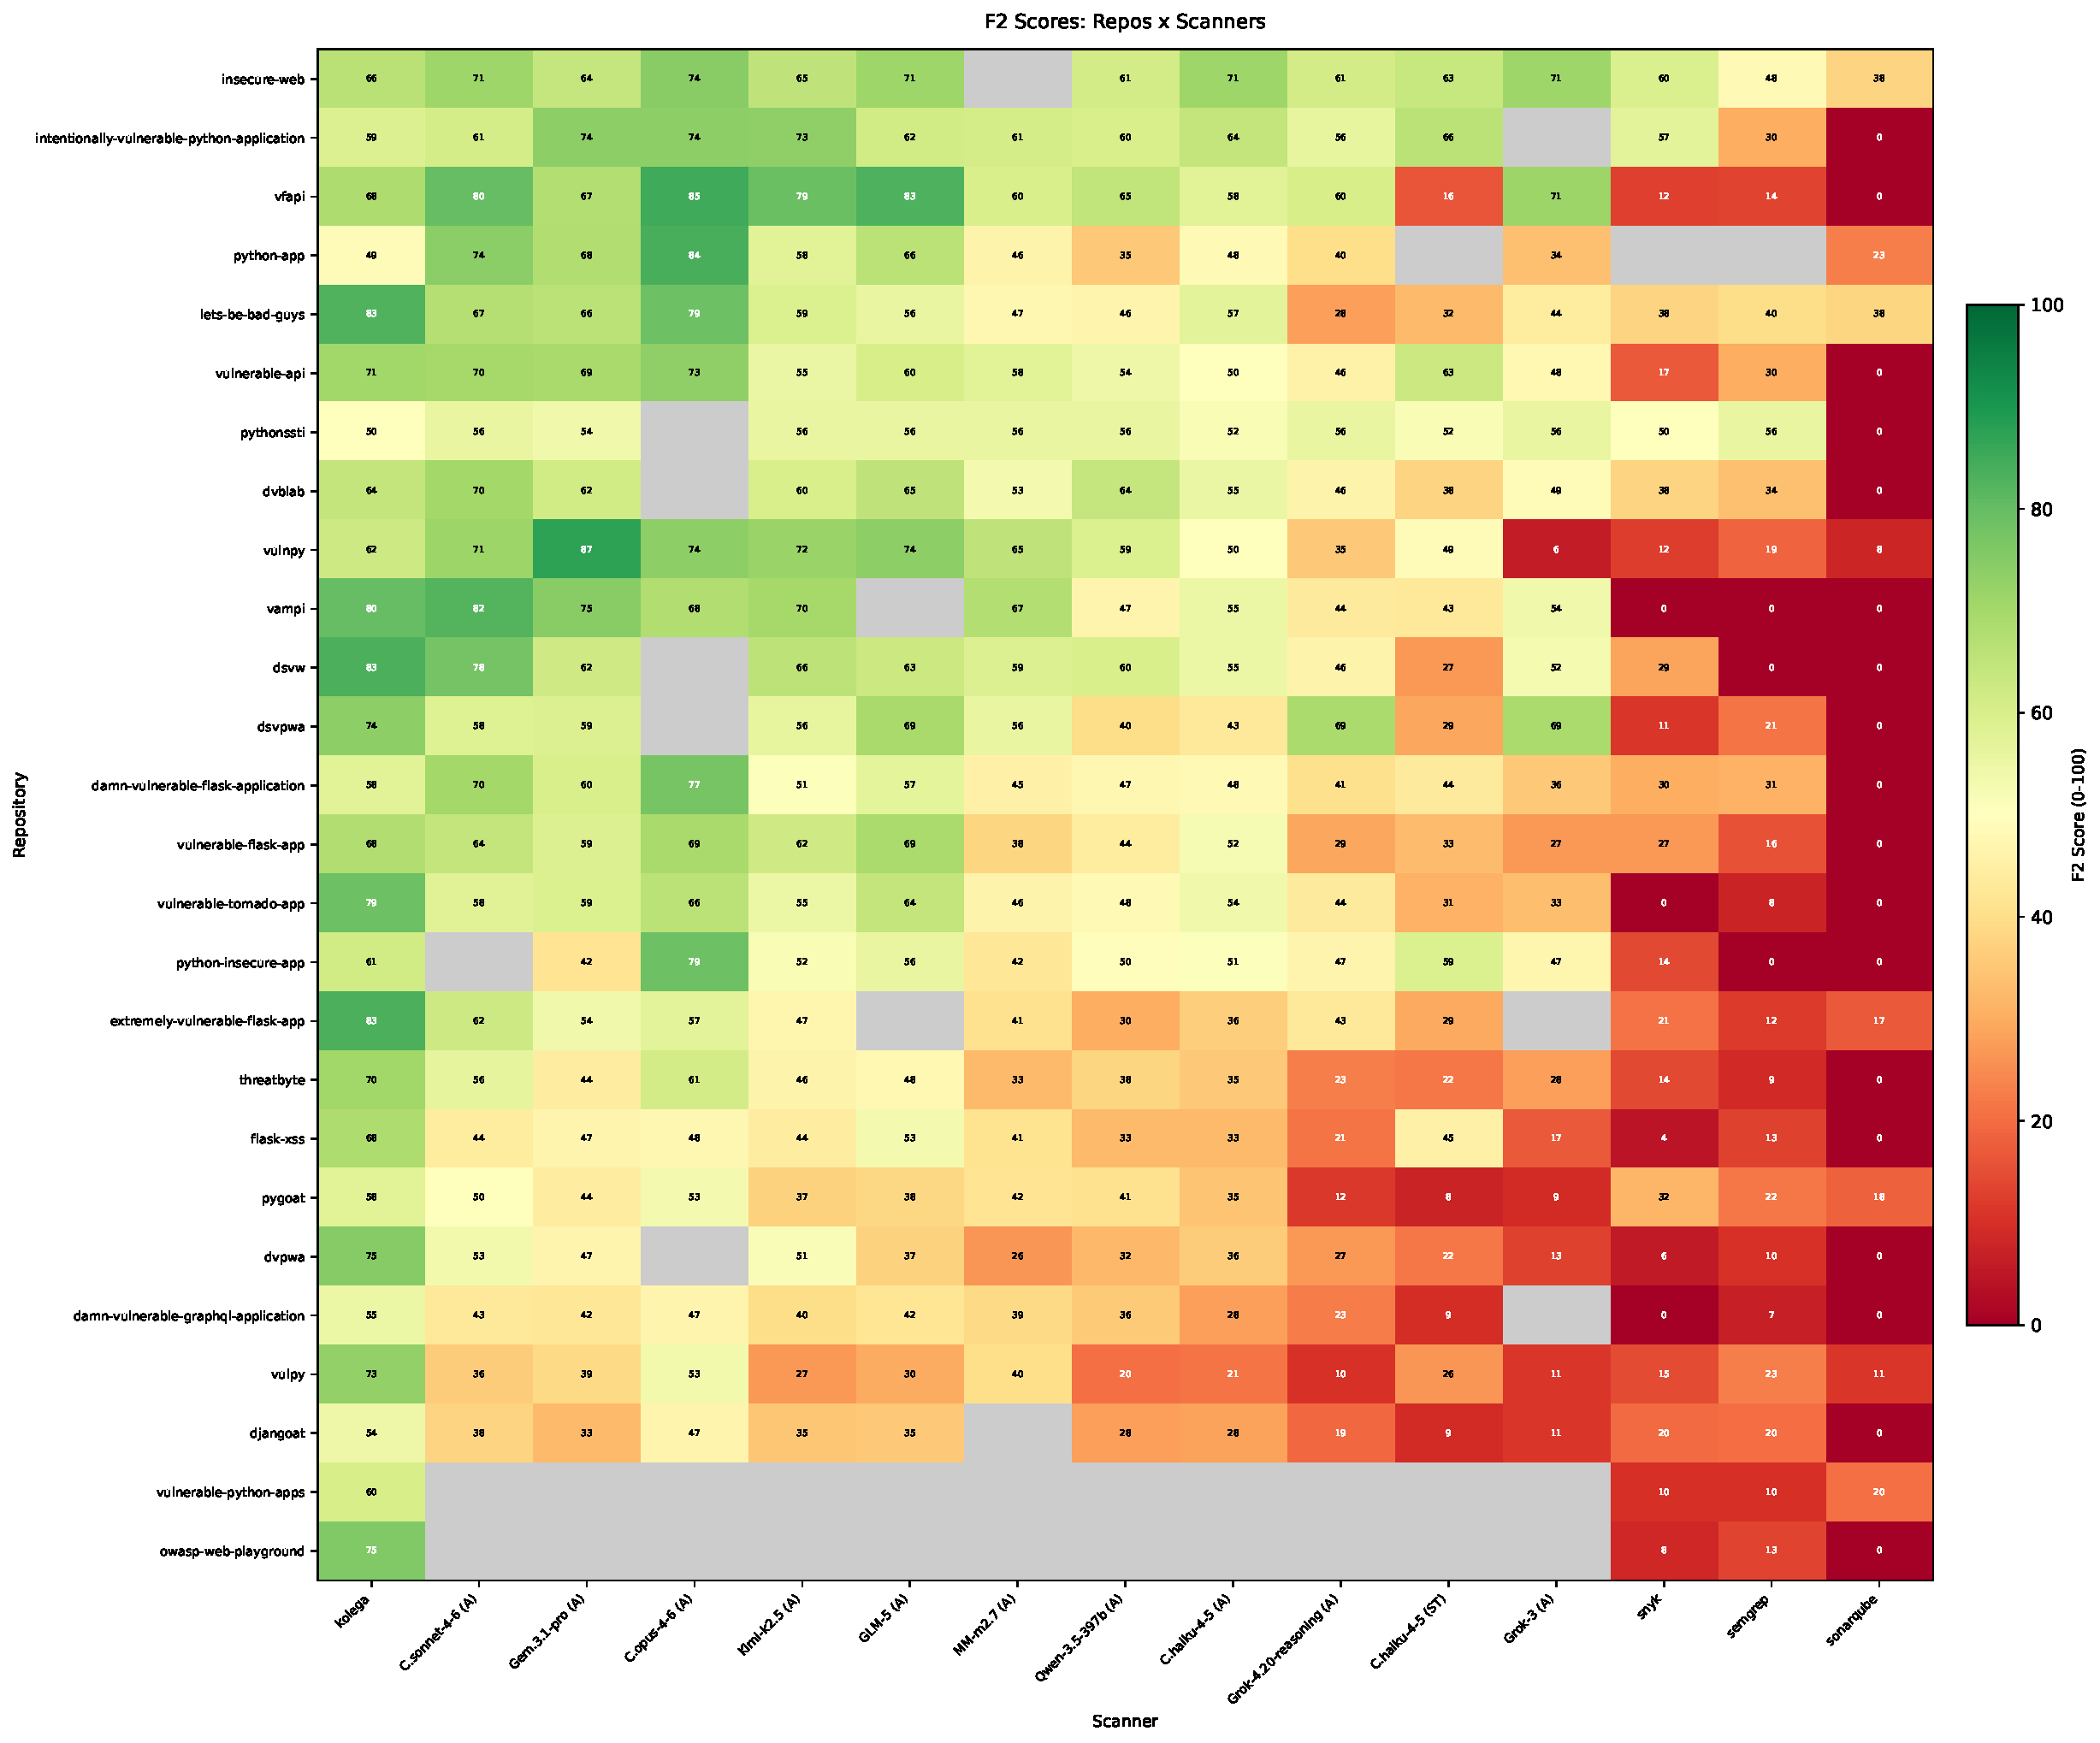
\includegraphics[width=\textwidth]{figures/heatmap.pdf}
\caption{Per-repo F3 scores across all 14 scanners and 26 repositories. Darker cells indicate higher F3; gray cells indicate the scanner did not complete that repo (timeout or crash). Repos are sorted by mean F3 (easiest at top); scanners are sorted by aggregate F3 (best at left).}
\label{fig:heatmap}
\end{figure*}

Figure~\ref{fig:heatmap} visualizes the full 26$\times$14 scoring matrix.
Several patterns emerge.

\textbf{Easy repos} such as \texttt{realvuln-pygoat} and \texttt{realvuln-dvpwa} are detected well by most scanners, including SAST tools, because they contain canonical vulnerability patterns (e.g., direct SQL string concatenation, unsanitized template rendering) that match existing rules.
\textbf{Hard repos}---those with low mean F3 across all scanners---tend to feature vulnerabilities requiring cross-file data-flow analysis or domain-specific knowledge (e.g., insecure deserialization in custom middleware, missing authorization checks in REST endpoints).
These repos differentiate LLM scanners from SAST: LLMs frequently score 40--70 on repos where SAST tools score 0--10.

The heatmap also reveals \textbf{high variance within LLM scanners}.
A model that excels on one repo may fail entirely on another of similar difficulty, suggesting that LLM-based vulnerability detection remains sensitive to codebase structure, naming conventions, and the specific vulnerability patterns present.
Gray cells (incomplete runs) cluster around the larger repos, confirming that \textbf{context-window limitations and timeout constraints} are practical bottlenecks for LLM scanners.

%% ─────────────────────────────────────────────
\subsection{Cost-Efficiency Analysis}
\label{sec:results:cost}

Table~\ref{tab:cost-efficiency} compares cost and detection performance across all scanner categories. Costs are normalized to \$/100k lines of code to enable direct comparison across different pricing models.

\begin{table}[t]
\centering
\caption{Cost-efficiency comparison. Costs normalized to \$/100k LOC. Rule-based SAST tools are free/open-source. Kolega pricing is \$25/100k LOC (published rate).}
\label{tab:cost-efficiency}
\footnotesize
\begin{tabular}{@{}llrr@{}}
\toprule
\textbf{Scanner} & \textbf{Cat.} & \textbf{F3} & \textbf{\$/100k LOC} \\
\midrule
Kolega v0.0.1        & Sec.-spec.  & \textbf{73.0} & \textbf{25} \\
\midrule
Claude Sonnet 4.6    & GP-LLM      & 51.7 & 83 \\
Gemini 3.1 Pro       & GP-LLM      & 51.0 & 136 \\
Claude Opus 4.6      & GP-LLM      & 47.5 & 123 \\
Kimi K2.5            & GP-LLM      & 46.5 & 11 \\
GLM-5                & GP-LLM      & 45.6 & 34 \\
Minimax M2.7         & GP-LLM      & 38.5 & 8 \\
Grok 4.20 Reasoning  & GP-LLM      & 27.5 & 84 \\
Grok 3               & GP-LLM      & 20.6 & 28 \\
\midrule
Semgrep              & Rule SAST   & 17.7 & 0 (free) \\
Snyk                 & Rule SAST   & 17.3 & 0 (free tier) \\
SonarQube            & Rule SAST   & 6.8  & 0 (free) \\
\bottomrule
\end{tabular}
\end{table}

\textbf{Kolega dominates the cost-efficiency frontier.} At \$25 per 100k LOC, it achieves the highest F3 (73.0) at a fraction of the cost of general-purpose LLM scanners. The best-performing GP-LLM (Claude Sonnet~4.6, F3\,=\,51.7) costs \$83/100k LOC --- \textbf{3.3$\times$ more expensive for 29\% lower F3}. The most expensive scanner (Gemini~3.1~Pro, \$136/100k LOC) achieves only F3\,=\,51.0, making it \textbf{5.4$\times$ more expensive than Kolega for 30\% lower detection}.

Among GP-LLM scanners, Kimi~K2.5 (\$11/100k LOC, F3\,=\,46.5) and Minimax~M2.7 (\$8/100k LOC, F3\,=\,38.5) offer the best value, but even these budget options score 36--47\% below Kolega.

Rule-based SAST tools are free but, as shown in Section~\ref{sec:results:aggregate}, detect fewer than 18\% of vulnerabilities --- a false economy when the cost of a missed vulnerability is measured in breaches rather than dollars.

%% ─────────────────────────────────────────────
\subsection{False-Positive Trap Effectiveness}
\label{sec:results:fp-traps}

\begin{figure*}[t]
\centering
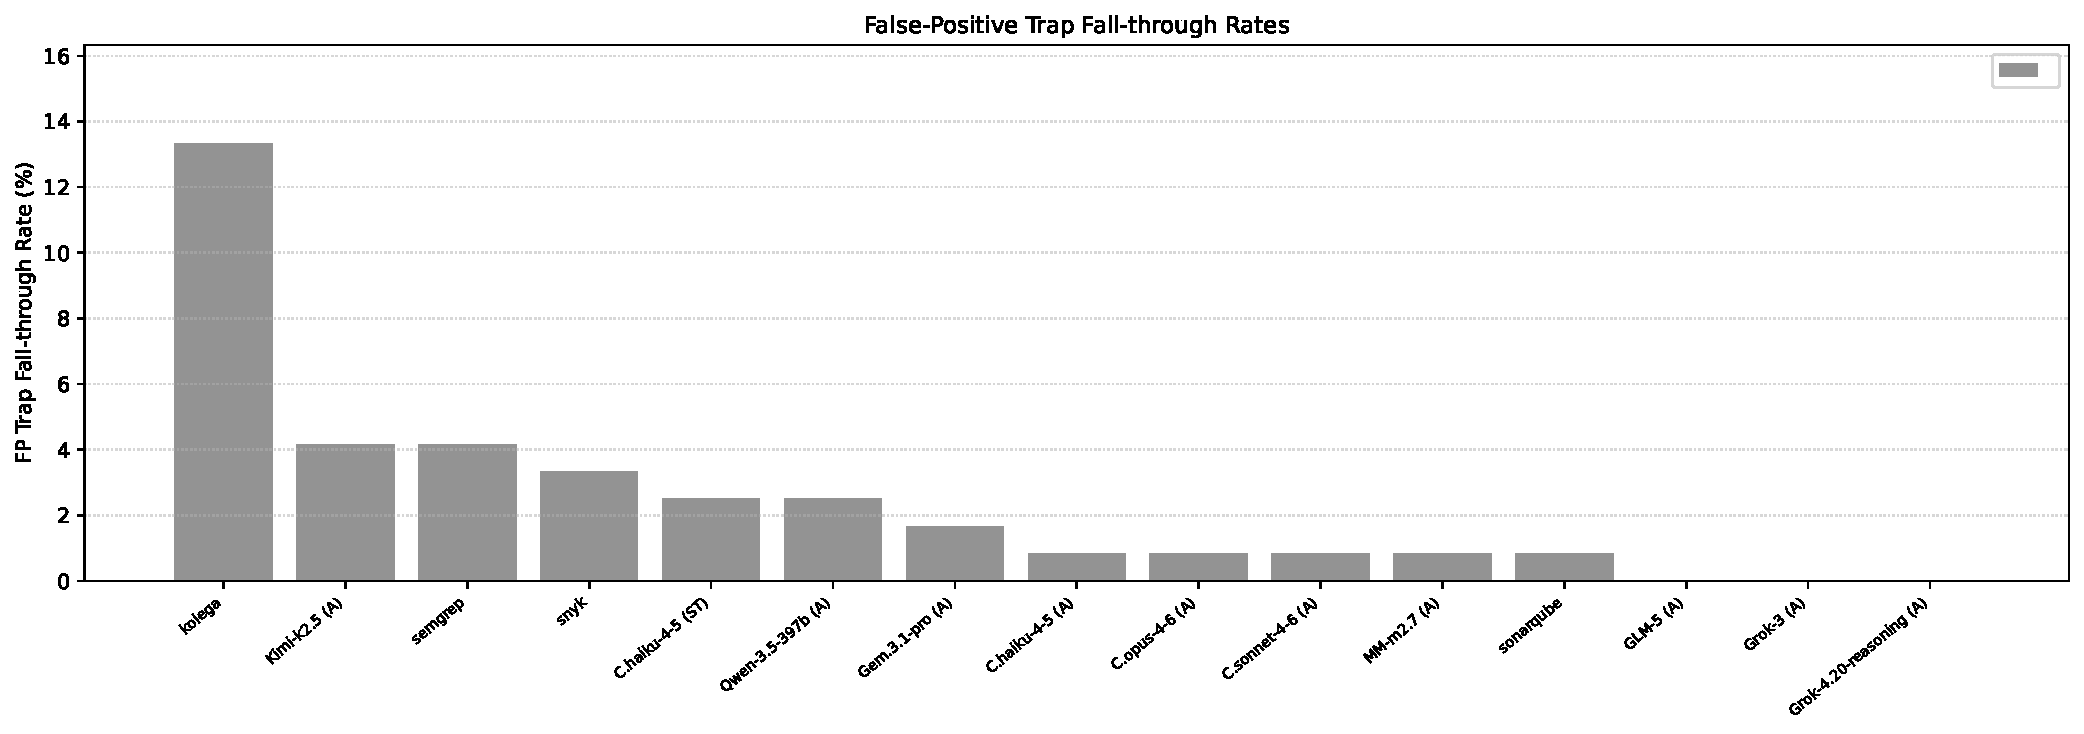
\includegraphics[width=\textwidth]{figures/fp-trap-rates.pdf}
\caption{False-positive trap trigger rates across scanners. The benchmark contains 120 FP traps---ground-truth entries marked \texttt{is\_vulnerable: false} that resemble real vulnerabilities. A scanner that flags these entries incurs a false-positive penalty.}
\label{fig:fp-traps}
\end{figure*}

The 120 false-positive traps embedded in RealVuln serve a dual purpose: they penalize scanners that over-report, and they validate that the benchmark discriminates between scanners with different precision characteristics.

Figure~\ref{fig:fp-traps} shows the trap trigger rate for each scanner.
\textbf{Rule-based SAST tools trigger FP traps at higher rates than LLM-based scanners.}
Semgrep, which relies on syntactic pattern matching, flags code constructs that superficially resemble vulnerabilities but are actually safe (e.g., parameterized queries that happen to include string formatting elsewhere in the function).
SonarQube's lower trigger rate reflects its conservative detection strategy---it fires few rules overall, reducing both true and false positives.

Among LLMs, the results validate the precision rankings from Table~\ref{tab:leaderboard}.
\textbf{Grok~4.20~Reasoning triggers the fewest traps}, consistent with its benchmark-leading precision of 0.927.
Conversely, Kolega triggers 16 of 120 FP traps (13.3\%), reflecting its high-recall operating point: its precision of 0.388 means it trades increased false alarms for broader detection coverage.

The FP traps prove effective at \textbf{differentiating scanners}: trap trigger rates span a wide range across the 14 evaluated tools, and they correlate inversely with measured precision ($r < -0.8$).
This validates the trap design methodology described in Section~\ref{sec:benchmark-design} and confirms that RealVuln's FP traps are a meaningful evaluation signal rather than noise.

\section{Analysis \& Discussion}
\label{sec:discussion}

This section interprets the comparative results across the three scanner
categories, identifies the key patterns that emerge from the evaluation, and
acknowledges the limitations and threats to validity that constrain
the conclusions we can draw.

%% ----------------------------------------------------------------
\subsection{Key Findings}
\label{sec:key-findings}

\paragraph{A clear three-tier hierarchy emerges.}
The most striking result is the emergence of three distinct performance
tiers.  The security-specialized scanner (Kolega, F3\,=\,73.0 strict)
substantially outperforms even the best general-purpose LLM (Sonnet~4.6,
F3\,=\,51.7), which in turn achieves nearly 3$\times$ the F3 score of
the best rule-based tool (Semgrep, F3\,=\,17.7).

This hierarchy suggests that general-purpose LLM reasoning, while a
major advance over pattern matching, is not sufficient for
production-grade vulnerability detection.  Purpose-built security
architecture---combining LLM reasoning with domain-specific
design---delivers meaningfully higher recall.

We note two important caveats. First, the security-specialized category currently contains only one system (Kolega); additional tools in this category would be needed to confirm a distinct performance tier rather than a single outlier. Second, the general-purpose LLM tier exhibits high internal variance, with F3 scores ranging from 20.6 (Grok~3) to 51.7 (Sonnet~4.6) --- a spread larger than the gap between the best GP-LLM and the best rule-based tool. Some GP-LLM scanners (Grok~3, Haiku single-turn) perform at or below rule-based SAST levels, suggesting that model choice and configuration matter as much as the LLM-vs-SAST distinction.

The per-CWE breakdown reveals where these advantages originate.
General-purpose LLMs dramatically outperform rule-based SAST on
vulnerability classes that require semantic understanding: SQL injection
(91\% vs.\ 32\% recall), command injection (78\% vs.\ 24\%), and
insecure deserialization.  Rule-based SAST tools remain competitive only
on issues that reduce to syntactic patterns (e.g., hardcoded secrets),
but even on those categories their overall recall remains low.

\paragraph{Security-specialized architecture closes the gap that general-purpose LLMs cannot.}
The 41\% F3 gap between Kolega (73.0) and the best general-purpose LLM (Sonnet~4.6, 51.7) warrants examination. General-purpose LLMs bring powerful code reasoning but lack security-specific optimizations: they receive a generic prompt, process code through a general-purpose context window, and produce findings without domain-specialized validation. Security-specialized systems can incorporate vulnerability-aware code analysis pipelines, security-specific retrieval and context assembly, and domain-optimized detection strategies that compound to produce meaningfully higher recall. Critically, Kolega achieves this while completing 26 of 26 repositories with zero timeouts --- demonstrating that purpose-built architecture solves the reliability problems that plague frontier general-purpose models (Opus: 36\% timeout rate, Minimax: 31\%). The combination of higher recall \emph{and} higher reliability is the defining advantage of the security-specialized category.

\paragraph{Where Kolega falls short.}
Despite leading the aggregate rankings, Kolega's precision of 0.388 is the lowest of any evaluated scanner --- meaning approximately 61\% of its findings are false positives. This is a substantial triage burden: for every true vulnerability found, an analyst must review roughly 1.6 additional false alarms. Teams with limited analyst bandwidth may reasonably prefer a higher-precision scanner such as Sonnet~4.6 (precision 0.785) at the cost of lower recall. Kolega also underperforms general-purpose LLMs on several individual repositories: on \texttt{realvuln-python-app} (Kolega F3\,=\,55.8 vs.\ Opus~4.6 at 83.5), \texttt{realvuln-vulnpy} (Kolega 62.6 vs.\ Gemini~3.1~Pro at 86.9), and \texttt{realvuln-damn-vulnerable-flask-application} (Kolega 67.0 vs.\ Opus~4.6 at 77.4). These repos suggest that Kolega's advantage is not universal --- on well-structured codebases with canonical vulnerability patterns, general-purpose LLMs can match or exceed it.

\paragraph{Agentic tool use is highly cost-effective.}
Comparing agentic and single-turn modes of the same underlying model
provides a controlled test of the value of tool use in vulnerability
detection.  Agentic Haiku achieves an F3 of 37.1 (strict) versus 25.2 for
single-turn Haiku---a 47\% improvement---while incurring only 6\% higher
cost.  The ability to read files, grep for patterns, and iteratively
explore a codebase allows the model to gather context that a single
prompt cannot provide.  This is consistent with the broader finding that
retrieval-augmented and tool-augmented LLM workflows outperform
prompt-only setups in code understanding tasks.  From a practical
standpoint, the marginal cost of agentic execution is small relative to
the gain in detection quality, making it the dominant strategy for
LLM-based scanning.

\paragraph{Bigger models do not always win; reliability matters.}
One might expect a monotonic relationship between model capability
(and cost) and benchmark performance.  The data tell a more nuanced
story.  Opus~4.6 achieves strong per-repo scores on the repositories
it completes, but its 36\% timeout rate (completing only 19 of 26
repos) drags its strict F3 down to 47.5---below Sonnet~4.6's 51.7,
which reflects fuller coverage.  A similar pattern emerges with
Minimax, which times out on 31\% of repos.  Conversely,
Kimi~K2.5 and Minimax~M2.7 punch above their weight on
cost-efficiency metrics, delivering competitive F3 scores at
substantially lower per-repo cost.  The implication for practitioners is
that scanner selection should optimize for \emph{reliability-adjusted}
performance rather than peak capability: a model that reliably completes
every scan is more valuable than one that occasionally excels but
frequently fails to return results.

\paragraph{The precision--recall tradeoff is stark and F3 captures it correctly.}
Grok~4.20 Reasoning exemplifies the conservative end of the spectrum:
its precision of 0.927 is the highest in the benchmark, but its recall
of 0.263 means it misses nearly three-quarters of true vulnerabilities.
Most LLM scanners cluster in the 0.6--0.8 precision range with
substantially higher recall, which the F3 metric---designed to weight
recall nine times more heavily than precision---correctly rewards.  Among
rule-based tools, SonarQube illustrates the opposite failure mode:
respectable precision (0.611) paired with negligible recall (0.065),
yielding an F3 of just 6.8.  The F3 metric aligns well with
practitioner priorities in security scanning, where a single missed
vulnerability can lead to a catastrophic breach while false positives
merely cost analyst time.  Benchmarks that report
only precision or only detection rate would paint a misleading picture
of scanner utility.

%% ----------------------------------------------------------------
\subsection{Limitations}
\label{sec:limitations}

We identify seven limitations that scope the conclusions of this work:

\begin{itemize}
  \item \textbf{Python only.}
    Version~1.0 of \textsc{RealVuln} covers only Python repositories.
    Scanner performance may differ substantially on statically typed
    languages (Java, Go) or memory-unsafe languages (C/C++) where
    vulnerability classes such as buffer overflows are prevalent.
    Extension to additional languages is planned for v2
    (Section~\ref{sec:living-benchmark}).

  \item \textbf{Type~1 repositories only.}
    All 26 repos are intentionally vulnerable applications with
    artificially high vulnerability density.  Production codebases have
    sparser vulnerabilities embedded in larger, more complex code, which
    may alter both precision and recall characteristics.  Type~2--5
    targets (Section~\ref{sec:target-types}) will address this gap.

  \item \textbf{Vendor conflict of interest.}
    Kolega, which leads the benchmark at F3\,=\,73.0 (strict), is also the
    organization publishing this work.  We mitigate this concern by
    open-sourcing the entire benchmark: ground truth labels, scoring
    code, scanner outputs, and the dashboard.  Any researcher can
    independently verify our results or challenge the ground truth.

  \item \textbf{Ground truth subjectivity.}
    Hand-labeling vulnerabilities inherently involves judgment calls,
    particularly for borderline cases such as informational findings or
    context-dependent misconfigurations.  We publish the labeling
    evidence and rationale for every ground truth entry and invite
    community challenges via the project's issue tracker.

  \item \textbf{LLM non-determinism.}
    LLM-based scanners produce variable output across runs.  We report
    multi-run statistics (mean, standard deviation) where available, but
    cost constraints prevented multi-run evaluation for every model
    configuration.  Single-run results should be interpreted with
    appropriate uncertainty.

  \item \textbf{Default scanner configurations.}
    All scanners are evaluated using default or vendor-recommended
    settings.  Tuned configurations---custom rules for Semgrep, adjusted
    quality profiles for SonarQube, or modified system prompts for
    LLM scanners---could yield different results.  We report the exact
    configuration used for each scanner to enable reproduction.

  \item \textbf{Timeouts and incomplete scans.}
    Opus~4.6 timed out on approximately 36\% of repositories and
    Minimax~M2.7 on approximately 31\%.  These incomplete scans reduce
    effective coverage and are reflected in the strict micro F3 metric,
    which treats unscanned repos as zero.  The gap between lenient and
    strict scores quantifies the reliability penalty.

  \item \textbf{Missing scanner families.}
    OpenAI models (GPT-4o, o3) are absent from this evaluation due to API restrictions on automated security scanning at the time of evaluation. Their inclusion would broaden the general-purpose LLM tier. Similarly, open-weight models (Llama, Mistral) are not evaluated. We plan to include both in v2.

  \item \textbf{Single-turn vs.\ agentic comparison is limited.}
    Only Claude Haiku~4.5 was evaluated in both single-turn and agentic modes. The 47\% F3 improvement we report is based on this single model pair; different models may benefit more or less from agentic scaffolding.
\end{itemize}

%% ----------------------------------------------------------------
\subsection{Threats to Validity}
\label{sec:threats}

\paragraph{Data contamination.}
The 26 target repositories are publicly available on GitHub, and it is
likely that some or all of them appeared in the training data of the LLM
scanners we evaluate.  If a model has memorized known vulnerabilities in
these repos, its recall could be inflated relative to performance on
unseen code.  We mitigate this threat in two ways.  First, the 120
false-positive traps in the ground truth test whether scanners
\emph{discriminate} between vulnerable and safe code; memorizing that a
file contains vulnerabilities does not help a scanner avoid flagging a
non-vulnerable code path in the same file.  Second, the v2 roadmap
(Section~\ref{sec:living-benchmark}) includes repositories published
after model training cutoffs, which will provide a contamination-free
evaluation set.

\paragraph{Selection bias.}
Twenty-six repositories, while substantial for a hand-labeled benchmark,
do not exhaustively represent the Python vulnerability landscape.
Certain CWE families (e.g., cryptographic weaknesses, race conditions)
are underrepresented in the current corpus.  The living-benchmark
roadmap addresses this through planned expansion to additional repos
and target types, aiming for broader CWE and application-domain
coverage in future versions.

\section{The Living Benchmark}
\label{sec:living-benchmark}

A static benchmark becomes stale as soon as the scanners it measures improve.
RealVuln is designed to grow alongside the tools it evaluates.

\subsection{Versioning and Community}

Every benchmark release is identified by a deterministic \emph{manifest hash} computed from ground-truth content, pinned repository commits, and prompt versions. Scores are always reported against a named manifest version. When new repositories or corrected labels are added, the hash changes and a new version tag is created. Old results remain valid, and the live dashboard at \url{https://realvuln.kolega.dev/} surfaces side-by-side comparisons against historical versions.

RealVuln is maintained as a community resource. Contribution pathways (adding repositories, submitting scanner results, and challenging ground-truth labels) are documented in the repository README.\footnote{\url{https://github.com/kolega-ai/RealVulnBenchmark}} The live leaderboard is rebuilt automatically on every merge to the \texttt{deploy\_pages} branch.

\subsection{Roadmap}

The following extensions are planned for v2:
\begin{itemize}
  \item \textbf{Multi-language expansion:} JavaScript/TypeScript, Go, and Java repositories.
  \item \textbf{Type~2 targets:} production apps with CVE-linked commits at realistic vulnerability density.
  \item \textbf{Type~3 targets:} vulnerable open-source libraries patched for disclosed CVEs.
  \item \textbf{Type~4 roll-ups:} OWASP Benchmark and Juliet re-scored under RealVuln metrics.
  \item \textbf{Agentic sandbox:} fully isolated, reproducible agentic evaluation via Docker containers.
\end{itemize}

\section{Conclusion}

We presented a systematic comparison of Rule-Based SAST tools, general-purpose
LLM scanners, and Security-Specialized systems, evaluated on
\textsc{RealVuln}, the first fully open-source benchmark built from real-world
vulnerable code.  Version~1 spans 26 repositories, 796 manually labeled
findings, and 120 false-positive traps across 15 scanners in three categories.
Every artifact (ground truth, raw scanner output, scoring pipeline, dashboard
generator, and evaluation prompts) is released under a permissive license
with a reproducible manifest that version-locks results to exact benchmark
snapshots.

Three tiers emerge clearly. The Security-Specialized scanner Kolega.Dev (F3\,=\,73.0 strict) leads, showing that purpose-built security architecture delivers higher recall than general-purpose methods. General-purpose LLM scanners form a competitive middle tier. The best, Claude Sonnet~4.6 (F3\,=\,51.7), scores nearly 3$\times$ higher than the best Rule-Based SAST tool, Semgrep (F3\,=\,17.7). No scanner dominates across all CWE families. Rule-Based tools retain a precision advantage on well-specified injection patterns. LLM-based systems do better on logic-level and authentication flaws that need broader code context. The contrast between the two Security-Specialized systems is instructive. The SecLab Taskflow Agent uses sophisticated multi-stage threat modeling with GPT-5.4 but scores F3\,=\,8.4, below every Rule-Based SAST tool. Its depth-first design audits only 3--5 threat categories per repository. Breadth of coverage, not just Security-Specialized architecture, separates the top tier from the rest. The future of vulnerability detection is not in applying general-purpose AI to security prompts. It is in building Security-Specialized systems that combine LLM reasoning with domain-specific architecture \emph{and} broad detection coverage.

The benchmark is designed to grow. New repositories, scanners, and ground-truth corrections can be added without invalidating prior results (\S\ref{sec:living-benchmark}).  Version 2 will expand coverage to JavaScript/TypeScript, Go, and
Java, and will introduce Type 2 targets drawn from real production CVEs,
setting a higher bar for precision in realistic, low-vulnerability-density
codebases.  We invite the security research community to submit scanner results,
propose new repositories, and challenge existing labels.

All code, data, results, and tooling are available at \url{https://github.com/kolega-ai/RealVulnBenchmark}. A live interactive dashboard is hosted at \url{https://realvuln.kolega.dev}. We encourage the security community to verify our results, challenge our ground truth, and submit their own scanner evaluations.


% === Acknowledgements ===
% \section*{Acknowledgements}
% TODO

\bibliographystyle{plainnat}
\bibliography{references}

% === Appendix ===
\appendix
\section{Matching Algorithm Pseudocode}
\label{sec:matching-pseudocode}

\begin{figure}[h]
{\footnotesize
\begin{verbatim}
MATCH(findings F, ground_truth G):
  matched_ids <- {}
  results <- []
  for each f in F:
    candidates <- []
    for each g in G:
      if g.id in matched_ids: continue
      if FILE_EQ(f, g) and CWE_IN(f, g)
         and LINE_OK(f, g):
        candidates.append(g)
    if candidates not empty:
      sort candidates: vuln=true first
      best <- candidates[0]
      matched_ids.add(best.id)
      if best.is_vulnerable:
        results.append(TP, best.id, f)
      else:
        results.append(FP, best.id, f)
    else:
      results.append(FP, null, f)
  for each g in G:
    if g.id not in matched_ids:
      if g.is_vulnerable:
        results.append(FN, g.id, null)
      else:
        results.append(TN, g.id, null)
  return results
\end{verbatim}
}
\caption{Pseudocode for the three-field matching algorithm. \texttt{FILE\_EQ} checks normalized path equality, \texttt{CWE\_IN} checks $\mathit{cwe}_f \in \mathit{cwes}_g$, and \texttt{LINE\_OK} checks line tolerance $\delta=10$.}
\label{alg:matching}
\end{figure}

\section{Ethics Statement}

All repositories evaluated in this benchmark are intentionally vulnerable
applications created explicitly for security education and training (e.g.\
PyGoat, DVPWA, VAmPI).  No responsible disclosure obligations arise from their
inclusion: the vulnerabilities they contain are by design, publicly documented,
and carry no risk of enabling attacks on production systems.  We publish no
zero-day vulnerability information and no novel exploitation techniques;
our ground-truth labels describe vulnerability \emph{classes} (CWEs) rather
than working exploit code.

Scanner weaknesses identified in our evaluation are disclosed in aggregate to
advance the state of the field.  We believe transparency about tool limitations
serves defenders more than it serves attackers, who can already assess scanner
efficacy empirically.

We acknowledge a potential conflict of interest: this benchmark is developed by
Kolega.Dev, a company that provides security tooling.  We mitigate this bias by
open-sourcing all benchmark artifacts (ground truth, scoring code, raw
scanner outputs, and evaluation harness) so that any party can audit our
methodology, re-run every evaluation, and verify reported scores independently.
Scanner results for Kolega.Dev-affiliated tools are held to the same evaluation
pipeline as all other entrants, with no post-hoc adjustment.

\section{Data Availability}

All artifacts described in this paper are publicly available under open licenses.

\begin{itemize}
  \item \textbf{Benchmark code} (MIT License) ---
    Scoring pipeline, parser library, and dashboard generator.

  \item \textbf{Ground truth} ---
    Hand-labeled vulnerability annotations for all 26 repositories.

  \item \textbf{Scan results} ---
    Raw output from all 15 evaluated scanners across every repository.

  \item \textbf{LLM evaluation harness} ---
    Prompt templates, agentic runner scripts, and per-run cost tracker.

  \item \textbf{Live dashboard} ---
    Interactive results explorer at \url{https://realvuln.kolega.dev}.

  \item \textbf{Benchmark manifest} ---
    Version-locked reproducibility file ensuring exact score reproduction.
\end{itemize}

\noindent All of the above are accessible at:
\url{https://github.com/kolega-ai/RealVulnBenchmark}


\end{document}
